\documentclass[tikz, border={0pt 0pt -2.99cm 0pt}]{standalone}
\usetikzlibrary{lindenmayersystems,decorations.pathreplacing,calc,arrows.meta}
\tikzset{
  % use of `show path construction` to draw all edges of the Lindenmayer systems
  edges/.style = {
    decoration={
      show path construction,
      lineto code={
        \draw[-{Stealth[scale=1]}, #1] ($(\tikzinputsegmentfirst)!.1!35:(\tikzinputsegmentlast)$)
        -- ($(\tikzinputsegmentlast)!.1!-35:(\tikzinputsegmentfirst)$);
      }
    },
    decorate
  },
  % define the Lindenmayer systems
  l-rect/.style = {
    l-system={rule set={F ->F[+F+F+F]f,f->ff}, axiom=F, order=#1,step=3cm},
  }
}
\begin{document}
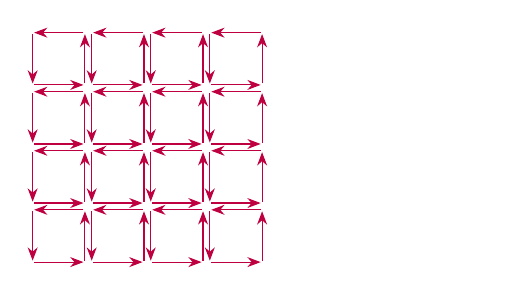
\begin{tikzpicture}[scale=0.25]
  \path[edges=purple] l-system [l-rect=3];
\end{tikzpicture}
\end{document}